\section{Эвристики для поиска кратчайших путей, алгоритм~A*.}

\begin{definition}
\textbf{Алгоритм А*} (англ. A star) — алгоритм поиска, который находит во взвешенном графе маршрут наименьшей стоимости от начальной вершины до выбранной конечной.
Данный алгоритм часто используется при поиске кратчайшего пути на плоскости.

Аналогично алгоритму Дейкстры работает только с графами с неотрицательными весами. 
\end{definition}

\subsection*{Эвристическая функция}

В процессе работы алгоритма для вершин рассчитывается функция  $f(v)=g(v)+h(v)$, где
\begin{itemize}
	\item $g(v)$ --- наименьшая стоимость пути в $v$
	из стартовой вершины,
	\item $h(v)$ --- эвристическое приближение стоимости пути от $v$ до конечной цели.
\end{itemize}

Функция $h(v)$ называется \textbf{допустимой}, если для любой вершины $v$ значение $h(v)$ меньше или равно весу кратчайшего пути от $v$ до цели.

Так же функция $h(v)$ должна быть \textbf{монотонной}

Первое условие является обязательным, при наличии второго условия алгоритм A* является \textbf{оптимальным}

Примеры эвристических функций $h(v)$ (будем считать, что вершины графа находятся на плоскости и у каждой есть координаты $(x, y)$)
\begin{enumerate}
	\item Если возможно перемещение в 4 направлениях, то в качестве эвристики выбирается \textbf{манхэттенское расстояние}
	$$h(v) = |v.x - goal.x| + |v.y - goal.y|$$
	\item \textbf{Расстояние Чебышева} применяется, когда к четырем направлениям добавляются диагонали
	$$h(v) = max\left(|v.x - goal.x|, |v.y - goal.y|\right)$$
	\item Если передвижение не ограничено сеткой, то можно использовать \textbf{евклидово расстояние} по прямой
	$$h(v) = \sqrt{(v.x - goal.x)^2 + (v.y - goal.y)^2}$$
\end{enumerate}

\subsection*{Сам алгоритм:}
\textbf{Инициализация}\\
Аналогично алгоритму Дейкстры:\\

Ищем путь из $s$ в $t$

Создаём приоритетную очередь $PQ$, в которую будем добавлять пары $(h(v), v)$ для всех вершин $v$, где $h(v)$ --- эвристическая оценка расстояния от $v$ до $t$.
В начале $PQ$ содержит только $(h(s), s)$. 
Массив $p[i] = -1$ --- для восстановления путей.

\textbf{Шаг алгоритма}\\
Пока $PQ$ не пуста:
\begin{enumerate}
	\item Извлекаем из $PQ$ вершину $u$ с минимальным значением $dist[u] + h(u)$ \textit{(единственное отличие от алгоритма Дейкстры)}
	\item Если $u = t$, то все пути найдены, завершаем работу алгоритма.
	\item Для каждого соседа $v$ вершины $u$:
	\begin{itemize}
		\item Если $dist[u] + w(u, v) < dist[v]$:
		\begin{itemize}
			\item $dist[v] = dist[u] + w(u, v)$.
			\item $p[v] = u$.
			\item Добавляем или обновляем $(dist[v] + h(v), v)$ в $PQ$
		\end{itemize}
	\end{itemize}
\end{enumerate}

\begin{figure}[h!]
	\centering
	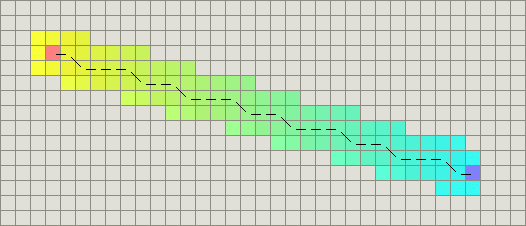
\includegraphics[width=0.7\linewidth]{img_easy/9_1.png}
	\captionsetup{labelformat=empty}
	\caption{Пример А* на сетке с возможностью ходить в восьми направлениях}
\end{figure}

\subsection*{Другие эвристики для поиска кратчайших путей}
\begin{enumerate}
	\item \textbf{Двунаправленный поиск} --- запуск алгоритма А* из начальной и конечной вершины сразу.
	Такая эвристика может значительно уменьшить количество посещённых вершин (в случае, если граф является ориентированным, поиск из конечной вершины запускается в противоположных рёбрах)
\end{enumerate}